%%%%%%%%%%%%%%%%%
%Mẫu làm khóa luận bằng LaTeX
%Soạn trên Texstudio
%Bộ gõ Unikey 4.0
%Người soạn: Nguyen Dang Chung Duc
%Liên lạc: nguyendangchungduc1999@gmail.com
%%%%%%%%%%%%%%%%%

\documentclass[12pt,a4paper]{report}
\usepackage[utf8]{vietnam}
\usepackage{amsmath, amsthm, amssymb,latexsym,amscd,amsfonts,enumerate}
\usepackage[top=2.0cm, bottom=2.5cm, left=3.0cm, right=2.0cm]{geometry}  % căn lề theo quy chuẩn KLTN
\usepackage{color, fancyhdr, graphicx, wrapfig}
\usepackage[unicode]{hyperref}
\usepackage{graphicx}

\newtheorem{dn}{Định nghĩa}[section]
\newtheorem{tc}[dn]{Tính chất}
\newtheorem{dl}[dn]{Định lí}
\newtheorem{md}[dn]{Mệnh đề}
\newtheorem{bd}[dn]{Bổ đề}
\newtheorem{hq}[dn]{Hệ quả}
\newtheorem{nx}[dn]{Nhận xét}
\newtheorem{vd}{Ví dụ}


\pagenumbering{roman}\pagestyle{plain}
\pagestyle{fancy}
\lhead{\it Báo cáo đồ án I}
\rhead{\it }
\lfoot{\it Nguyễn Quang Huy} 			         
\rfoot{\it ĐTVT03-K62}
\renewcommand{\headrulewidth}{1,2pt} 			
\renewcommand{\footrulewidth}{1,2pt}   % Cái này là tiêu đề chạy

\begin{document} 

\fontsize{13pt}{18pt}\selectfont   % Lệnh thay đổi cỡ chữ thành cỡ 13, cỡ dòng 18 (theo quy chuẩn của Khóa Luận TN).

\setlength{\baselineskip}{18truept}
\begin{titlepage}                                                       % Đây là trang bìa
\begin{center}
{\large\bf TRƯỜNG ĐẠI HỌC BÁCH KHOA HÀ NỘI}\\
{\large\bf VIỆN ĐIỆN TỬ - VIỄN THÔNG} \\
{---------------------o0o--------------------}
\vskip 2cm

\begin{center}
	
\includegraphics[scale=.2]{logo_hust.jpg}	
\end{center}

{\bf BÁO CÁO TIẾN ĐỘ TRIỂN KHAI ĐỒ ÁN I}\\[1cm]
{\Large\bf \textbf{ĐỊNH VỊ VÀ BÁM ĐỐI TƯỢNG CHUYỂN ĐỘNG BẰNG XỬ LÝ VIDEO TỪ UAV}}\\
\vskip 1cm
%{\bf {\it Chuyên ngành:}  Phương trình vi - tích phân}
\vskip 1cm

\begin{tabular}{r l}
Giảng viên hướng dẫn:&{\bf TS. Phạm Văn Tiến}\\[0.5cm]
Sinh viên:&{\bf Nguyễn Đặng Chung Đức} \\ &{\bf Nguyễn Quang Huy}\\[0.5cm]
%MSSV:&{\bf 20172484}\\[0.5cm]
%Lớp:&{\bf ĐTVT11\-K62}
\end{tabular}
\vfill
{\bf HÀ NỘI, 11/2020}
\end{center}
\end{titlepage}



\chapter*{\centering{LỜI NÓI ĐẦU}}
\vskip 1cm
\addcontentsline{toc}{chapter}{{\bf Lời nói đầu}\rm} %Đưa lời nói đầu vào mục lục
\hspace{25pt}Sau khi tiến hình lập trình mô phỏng quá trình cất cánh, hạ cánh, chuyển động theo quỹ đạo được thiết kế từ trước trên FLytsim, nhóm dự định sẽ cho bay thực tế, tuy nhiên thiết bị bay chỉ có thể duy trì từ 2-3 phút, nên công việc này đang tạm trì hoãn, tuần này nhóm tiến hành stream video thu được từ camera CSI gắn trên Pi qua laptop cá nhân dựa trên Ad Hoc Wifi, đây cũng là 1 phương án khả thi có thể giúp trạm mặt đất thu video từ camera trên UAV trong lúc phương án sử dụng telemetry vẫn chưa thể thống nhất do việc tìm kiếm telelemetry. Để đón đầu khi mà UAV có thể cải thiện thời gian bay, nhóm cũng tiến hành xây dựng thuật toán định vị đối tượng trong video thu được từ máy tính nhúng trên UAV dựa trên GPS của nó. 

\chapter*{\centering{MỘT SỐ KÝ HIỆU VIẾT TẮT}}
\vskip 1cm
\addcontentsline{toc}{chapter}{{\bf  Một số kí hiệu viết tắt}\rm} 
\begin{tabular}{l l }
RPI & Raspberry Pi.\\
UAV & Unmanned Aerial Vehicle.\\
GPS & Global Positioning System.\\
\end{tabular}

\tableofcontents
	                        % Lệnh mục lục
\chapter{KIẾN THỨC CƠ BẢN}         % Chương 1
\pagenumbering{arabic}                      % Đánh lại trang

\section{Giới thiệu về Ad Hoc}
\hspace{25pt} Ad hoc có thể được hiểu là vì mục đích xây dựng 1 mạng kết nối (chủ yếu là vô tuyến) giữa các thiết bị đầu cuối mà không cần phải dùng các trạm thu phát gốc. Nó cho phép các nút mạng truyền trực tiếp với nhau sử dụng bộ thu phát không dây mà không cần bất cứ cơ sở hạ tầng cố định nào. Dựa trên công nghệ ad hoc, các thiết bị cầm tay (điện thoại di động, PDA, laptop …) và các thiết bị cố định( các trạm cơ sở, các điểm truy cập internet không dây …) có thể được kết nối với nhau và tạo thành mạng toàn cầu.
\begin{figure}
	\begin{center}
		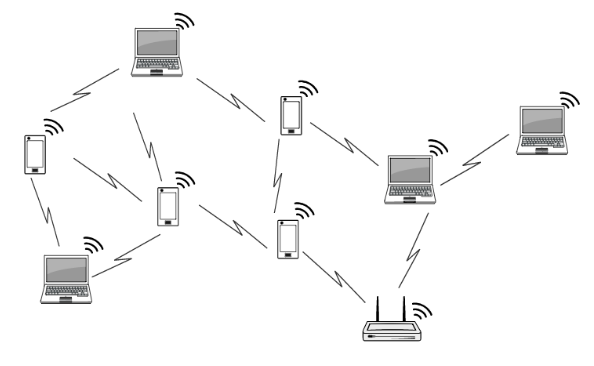
\includegraphics[scale=0.6]{ad_hoc.png}	
	\end{center}
	\caption{Wireless Ad Hoc Network}
	\label{refhinh1.1}\
\end{figure}

\section{Wireless Ad Hoc Network}
\hspace{25pt} Đây là 1 mạng không dây phân tán, mạng này không dựa trên cơ sở hạ tầng có sẵn từ trước như router trong mạng có dây hay điểm truy cập ngẫu nhiên trong những mạng không dây được quản lý. Thay vào đó, mỗi thiết bị (nút) tham gia định tuyến mạng bằng cách chuyển tiếp dữ liệu cho nút khác, vì thế việc quyết định nút nào chuyển tiếp dữ liệu được thực hiện tự động dựa trên cơ sở kết nối mạng và thuật toán định tuyến được sử dụng. Hay có thể hiểu đơn giản là ta có thể thiết lập kết nối không dây trực tiếp với máy tính hoặc thiết bị khác mà không cần kết nối với router hoặc điểm truy cập Wi-fi.

\begin{center}Adhoc
\begin{figure}[htp]
	\begin{center}
		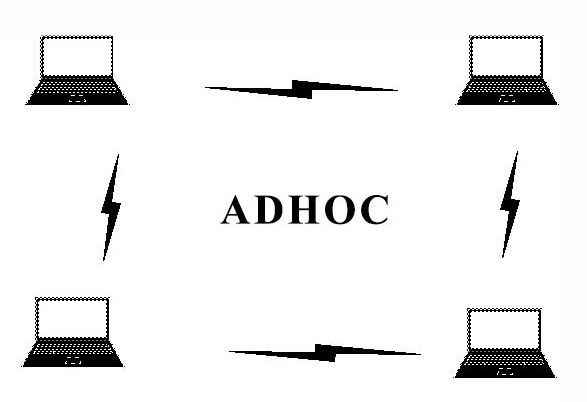
\includegraphics[scale=.6]{Ad.png}
	\end{center}
	\caption{Adhoc}
	\label{refhinh1}
\end{figure}
\end{center}

\section{Ưu điểm}
\begin{itemize}
	\item Mạng Ad Hoc được hợp thành từ các thiết bị không đồng nhất, các thiết bị như điện thoại di động, PDA, laptop…có thể liên lạc với nhau qua mạng Ad hoc
	\item Mạng Ad Hoc không yêu cầu điểm truy cập, nó cung cấp phương thức giao tiếp trực tiếp giữa các thiết bị
	\item Mạng Ad Hoc dễ dàng định cấu hình và cung cấp một cách hiệu quả để giao tiếp với các thiết bị lân cận khi điều cốt yếu là thời gian và việc chạy cáp là không khả thi
	\item Mạng Ad Hoc liên kết một số lượng nhỏ thiết bị có thể tốt hơn mạng thông thường với nhiều người dùng được kết nối hơn
\end{itemize}

\newpage         % Mấy lệnh \newpage và abc, xyz này khi gõ thì các bạn bỏ đi nhé!
\chapter{CÔNG VIỆC TRIỂN KHAI}                    % Chương 2
\section{Tiến hành cài đặt cho máy tính nhúng}
\subsection{Tiến hành thiết lập Ad Hoc Wifi và stream video trên RPI }
\begin{itemize}
	\item RaspberryPi 3 mà nhóm đang sử dụng được tích hợp chip wifi Broadcom, giúp ta dễ dàng thiết lập Ad Hoc Wifi
	\item Sau đó, ta sử dụng laptop cá nhân, đóng vai trò là trạm mặt đất, truy cập vào Wifi mà RPI vừa phát ra 
	\item Tiến hành cài đặt opencv trong môi trường ảo trên RPI
	\item Tiến hành xây dựng chương trình stream video từ RPI sang laptop cá nhân trong 60s với kích thước khung hình là 640x360
	\item Tiến hành kết nối camera CSI cho RPI, chỉnh sửa chất lượng video RPI để đạt được chất lượng phù hợp, chạy code và quan sát kết quả
\end{itemize}
\subsection{Kết quả thu được}
\begin{itemize}
	\item Video thu được đạt chất lượng đủ tốt để phục vụ mục đích của nhóm, tuy nhiên trong quá trình stream xảy ra hiện tượng trễ truyền, thời gian trễ tỉ lệ nghịch với kích thước khung hình
	\item Video thu được: https://drive.google.com/drive/folders/1G-HXXbuEE2KHUpaKngO-bvXtoh7KBmtC
		
\end{itemize}
\section{Xây dựng thuật toán định vị đối tượng}
\hspace{25pt} Nhóm đã tiến hành lập trình xong thuật toán định vị đối tượng, sang tuần, nhóm sẽ bay UAV và kiểm nghiệm tính chính xác của thuật toán ngoài thực tế, sau đó sẽ trình bày chi tiết về thuật toán. Hiện tại, nhóm chỉ nêu phần cốt lõi của giải thuật:
\begin{itemize} 
	\item Dựa vào độ cao, góc mở camera cùng với GPS của UAV, ta có thể xác định được chính xác kích thước khung hình thực tế mà UAV thu được
	\item Dựa vào các yếu tố trên, ta cũng tính chính xác khoảng cách thực tế của đối tượng với tâm khung hình thu được 
	\item Dựa vào góc lệch giữa khung hình khi UAV trong trạng thái lý tưởng và thực tế, cũng như hình chiếu của đối tượng trên khung hình thực tế và GPS của UAV, ta hoàn toàn có thể tính được GPS của đối tượng trong khung hình
	\item Sau khi thu được GPS của vật thể, ta gửi vị trí và lệnh điều khiển cho UAV, để UAV có thể bám theo đối tượng đó dựa trên GPS vừa thu được 
\end{itemize}

\chapter*{\centering{KẾT LUẬN}}                         % Chương 3
\addcontentsline{toc}{chapter}{{\bf  Kết luận}\rm}
\hspace{25pt} Video thu được qua stream từ camera CSI gắn trên RPI đạt chất lượng đủ tốt để phục vụ mục đích của nhóm, tuy nhiên trong quá trình truyền video, xảy ra hiện tượng trễ truyền, nhóm sẽ tiến hành xem xét và khắc phục nếu có thể, song song với đó, nhóm cũng sẽ đẩy mạnh công tác tìm kiếm telemetry phù hợp để điều khiển thiết bị bay và lập trình xử lý tín hiệu video trong quá trình hoạt động của UAV.\\
Vấn đề thời gian bay của UAV luôn là câu hỏi hóc búa làm nhóm trăn trở, tuần tới, nhóm sẽ tích cực tiến hành tìm hiểu và cải thiện thời gian bay cho UAV, đồng thời triển khai thuật toán định vị đối tượng để kiểm nghiệm tính chính xác ngoài thực tế, cũng như điều khiển UAV tự động dựa vào các chương trình nhóm đã lập trình sẵn trước đó từ các API của flybase

\begin{thebibliography}{99}               % Tài liệu tham khảo   
\addcontentsline{toc}{chapter}{{\bf  Tài liệu tham khảo}\rm} 

\bibitem{Eva} https://github.com/simondlevy/RPiAdHocWiFi
\bibitem{Eva} https://searchmobilecomputing.techtarget.com/definition/ad-hoc-network
\bibitem{Eva} https://timviec365.vn/blog/ad-hoc-la-gi-new5315.html
\bibitem{Eva} https://timviec365.com.vn/ad-hoc-la-gi-b453.html
\bibitem{Eva} https://wikihoidap.org/ad-hoc-la-gi
% Chú thích: mỗi tài liệu là một bibitem.

\end{thebibliography}


\end{document}

%Một số chú ý:
%-Sau phần \end{document} thì văn bản không còn hiển thị.
%-Các siêu liên kết (tên PT, định lí... được tham chiếu) thường có ô vuông đỏ bao quanh. Các bạn yên tâm, khi in ra sẽ ko xuất hiện cái ô vuông đó!